\section{Fine preconditioner : overlapping additive Schwarz}

Let us now move on the fine part of the preconditioner, $P^f$. As explained before, it consists of an OAS preconditioner. The general idea is to solve problem \ref{eq:poisson} with homogeneous Dirichlet boundary conditions on several subdomains that overlap and with the residual as the right-hand side. The results are subsequently added to form the fine scale preconditioner. 

The procedure explained here is to a large extend inspired from \cite{remacle}, we only adapt it to handle hanging nodes. 

\subsection{Overlapping subdomains}

\begin{figure}
\centering
\begin{subfigure}{.5\textwidth}
  \centering
  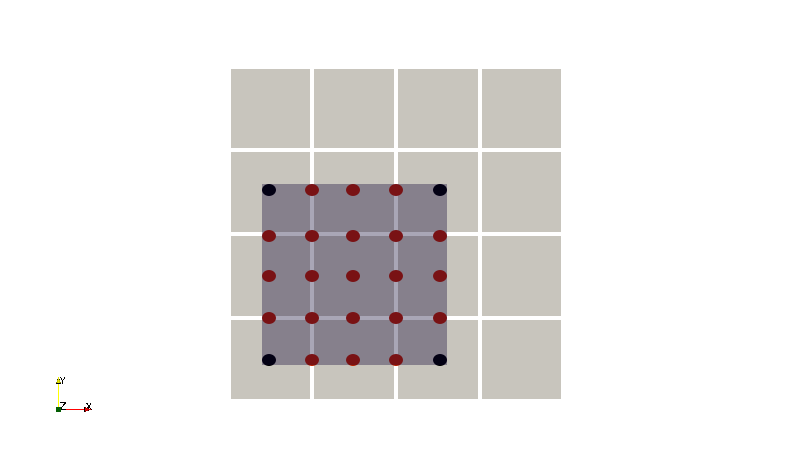
\includegraphics[width=1.2\linewidth]{Theory/fine_over_1.png}
  \caption{Subdomain for $p=2$ on a conforming mesh}
  \label{fine_over_1}
\end{subfigure}%
\begin{subfigure}{.5\textwidth}
  \centering
  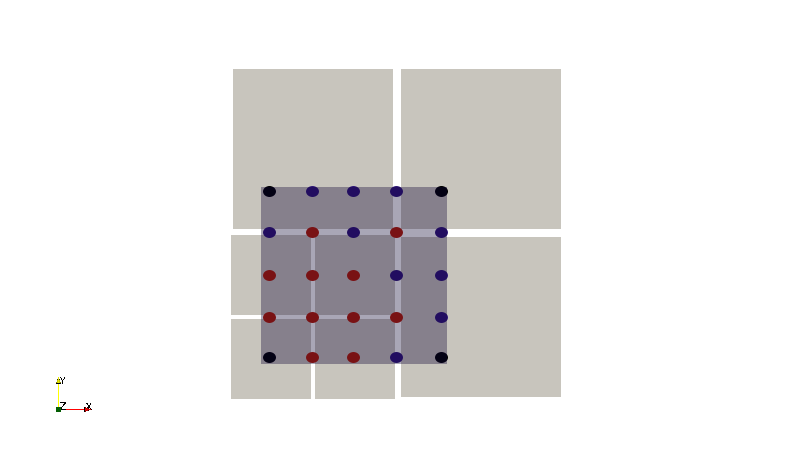
\includegraphics[width=1.2\linewidth]{Theory/fine_over_2.png}
  \caption{Subdomain for $p=2$ on a non conforming mesh}
  \label{fine_over_2}
\end{subfigure}
\caption{Example of two subdomains for $p=2$ used in the overlapping Schwarz preconditioner. On the left, we have a conforming mesh and all the local nodes are also global nodes (red). On the right, we have a non conforming mesh. Some nodes coincide with global GLL nodes (in red) but for others (in blue), we must use an interpolation to get their value. For both, the nodes at the corners of the subdomain (in black) will not be considered.}
\label{fine_over}
\end{figure}

We need to divide the mesh into overlapping subdomains. A natural choice is to use the quadrants and add a layer of GLL nodes to each side from neighboring quadrants. That yields $(p+3)^2$ local nodes on each subdomain. 

An example of the subdomains for $p=2$ is given in figure \ref{fine_over}. On the left, the mesh is conforming. That means that all the local nodes on subdomain $s$ coincide with global nodes. However, in a non conforming mesh, in addition to hanging nodes on some edges, we also need to interpolate the residual when, as presented in figure \ref{fine_over_2}, we are hanging with respect to our neighbor. There is also need for interpolation when at least one of our neighbor has hanging nodes. We can see here that adding hanging nodes brings a lot of new complexities. We will explain in more detail how they are treated in the implementation chapter. 

For now, let us assume that we have an operator $T_{ij;s}$ that gives the value of the local residual at local node $(i,j)$ on subdomain $s$. If we denote the global residual by $r$ and its restriction on subdomain $s$ by $r_{ij;s}$, then we have : 

\begin{align*}
r_{ij;s} &= T_{ij;s}r &\text{for $i,j=-1,0,...,p,p+1$} 
\end{align*}

Let us also note that, even in the conforming case, it is not always possible to compute the residual at the four corners of the subdomain (nodes in black on figure \ref{fine_over_1}). That is because in an unstructured mesh, a quadrant can have several other quadrants as neighbors through a corner or none at all. Therefore, we will impose that :

\begin{align*}
r_{ij;s} &= 0  &\text{at the four corners of the subdomain}
\end{align*} 

\subsection{Additive Schwarz method}

A more detailled explanation of the additive Schwarz method and the domain decomposition can be found in \cite{fine_book}. As said earlier, we now want to solve problem \ref{eq:poisson} to get the local fine scale correction, denoted by $z_{ij;s}$. In order to do this, we will impose homogeneous Dirichlet boundary conditions on nodes located at $i,j = -2$ or $i,j= p+2$.

As explained in \cite{over_acc}, since we are using the additive Schwarz method as a preconditioner, we do not need to be extremely accurate in the solution of problem \ref{eq:poisson}. We will also make an assumption that will allow us to compute the fine scale correction efficiently : we will assume that every quadrant is aligned with the axes. That means that a lot of geometric factors cancel and we can actually solve the problem analytically. We will see in the results chapter that, in practice, we can indeed make this assumption.

Let us first consider the equivalent 1D problem for an element of length $h$. The stiffness matrix is then given by : 

$$A^e_{ij} = \int_0^h  \frac{dl_i}{dx}\frac{dl_j}{dx} dx \approx \frac{2}{h} \sum_{m=0}^p w_mH_{im}H_{jm} = \frac{2}{h} d_{ij}$$

The influence of the overlaps (points at $-1$ and $p+1$) is computed using the standard finite element procedure : by adding their contribution to the stiffness matrix. We also assume that the neighboring elements have the same size so that the factor $h$ does not change. As a result, the linear system we obtain with the discretization is given by : 

\begin{align*}
A&= \begin{pmatrix}
d_{11} & d_{01} & 0 & \hdots & \hdots &\hdots & 0\\
d_{10} & 2d_{00} & d_{01} & \hdots & \hdots & d_{0p} & 0 \\
0 & d_{10} & d_{11} & \hdots & \hdots & d_{1p} & 0\\
\vdots & \vdots & \ddots & \ddots & \ddots & \vdots &\vdots \\
0 & d_{p-1,0} & \hdots & \hdots & d_{p-1,p-1} & d_{p-1,p} & 0\\
0 & d_{p0} & \hdots & \hdots & d_{p,p-1} & 2d_{pp} & d_{p-1,p}\\
0 & \hdots & \hdots & \hdots & 0 & d_{p,p-1} & d_{p-1,p-1}
\end{pmatrix}\\
M &= \begin{pmatrix}
w_1 & & & & & & \\
& 2w_0 & & & & & \\
& & w_1 & & & & \\
& & & \ddots & & &\\
& & & & w_{p-1} & &\\
& & & & & 2w_p & \\
& & & & & & w_{p-1}
\end{pmatrix}\\
\frac{4}{h^2}M^{-1}A z &= \frac{2}{h}M^{-1}r
\end{align*}

As mentioned in \cite{remacle}, the matrix $L = M^{-1}A$ is diagonalizable and it has real and positive eigenvalues $\lambda_i$. So let us define : 

$$ L = V^{-1}\Lambda V$$

That leads to an analytic solution for $z$. Indeed : 

$$ z = \frac{h}{2} V^{-1}\Lambda^{-1}V M^{-1}r$$

Let us now try to generalize this procedure to the two dimensional case. As explained before, let us assume that the subdomain $s$ is aligned with the axes $x$ and $y$ and has dimensions $h_x$ and $h_y$. Then the system of equations we have to solve to find the local fine scale correction on subdomain $s$, $z_{ij;s}$, is given by : 

\begin{align}
\sum_{m=-1}^{p+1} \frac{4}{h_x^2}L_{im}z_{mj;s} + \frac{4}{h_y^2} L_{jm}z_{im} &= \frac{4}{h_xh_y}\frac{1}{M_{ii}M_{jj}} r_{ij;s}  &\text{for $i,j=-1,...,p+1$} \label{eq:fine}
\end{align}

The reader can compare equation \ref{eq:fine} with the one derived in the section about the spectral element method to convince himself that it is indeed the set of equations obtained when the quadrant is aligned with the axes. 

Let us define the matrices $Z_s$ and $R'_s$  such that $(Z_s)_{ij} = z_{ij;s}$ and $(R'_s)_{ij} = \frac{4}{h_xh_y}\frac{1}{M_{ii}M_{jj}} r_{ij;s}$. Then, equation \ref{eq:fine} can be written as :

$$\frac{4}{h_x^2} LZ_s + \frac{4}{h_y^2} Z_sL^T = R'_s$$

Using the diagonalization of $L$, we have :

\begin{align}
\frac{4}{h_x^2} V^{-1}\Lambda V Z_s + \frac{4}{h_y^2} Z_s V^T\Lambda V^{-T} &= R'_s \nonumber \\
\frac{4}{h_x^2} \Lambda VZ_sV^T + \frac{4}{h_y^2} VZ_sV^T \lambda &= VR'_sV^T \label{eq:fine_inter}
\end{align}

Let us define $W = VZ_sV^T$ and $D=VR'_sV^T$. Then, it is obvious that the solution to equation \ref{eq:fine_inter} is given by : 

\begin{align*}
W_{ij} &= \frac{1}{\frac{4}{h_x^2}\lambda_i + \frac{4}{h_y^2}\lambda_j}D_{ij} &\text{for $i,j=-1,...,p+1$}\\
Z_s &= V^{-1}WV^{-T}
\end{align*}

We have reduced the problem to a few matrix products (where the matrices have $(p+3)$ rows and columns). If we had taken the geometric factors into account, we would have had a system with $(p+3)^2$ unknowns to solve for each subdomain $s$. That is $\mathcal{O}((p+3)^6)$ operations using a direct method. Here, we only need to perform matrix products and therefore we need $\mathcal{O}((p+3)^3)$ operations. The gain would be even greater in three dimensions. Let us note that the diagonalization of $L$ can be done once at the beginning since it does not depend on the subdomain.

The last thing we have to do is to gather the local fine preconditioner to the global GLL nodes to form the global fine preconditioner. As before, the gather operator is the transpose of the restriction operator. That yields : 

$$ P^f r = \sum_s \sum_{i=-1}^{p+1}\sum_{j=-1}^{p+1} T^T_{ij;s} z_{ij;s}$$

\subsection{Managing the actual boundary}

Up until now, we have assumed that the subdomain was included in $\Omega$. But some quadrants have at least an edge on $\Gamma$. In order to be able to use the analytic solution described above, we however need to give a value to the local fine residual. 

The method used here is to interpolate the value of the residual from inside the domain. For example, if the south edge is on the boundary $\Gamma$, then the local fine residual is given by : 

\begin{align*}
r_{i,-1;s} &= 2r_{i,0} - r_{i,1} &\text{for $i=0,...,p$}
\end{align*}

Of course, we do not gather the value of the fine scale correction that is outside of $\Omega$.









